\documentclass[aspectratio=169,10pt]{beamer}

\usetheme{default}
\usecolortheme{default}
\setbeamertemplate{navigation symbols}{}
\setbeamertemplate{footline}[frame number]
\setbeamertemplate{itemize items}[circle]
\setbeamercolor{alerted text}{fg=blue!55!black}
\setbeamerfont{frametitle}{size=\large,series=\bfseries}

\usepackage{amsmath,amssymb,mathtools}
\usepackage{booktabs,array}
\usepackage{graphicx}
\usepackage{tabularx}
\usepackage{microtype}

\graphicspath{{assets/}}
\newcommand{\takeaway}[1]{\vfill{\footnotesize\textbf{Takeaway.} #1}}
\newcommand{\notfound}[1]{\textbf{[NUMBER NOT FOUND: #1]}}

\title{[PLACEHOLDER: Title TBD]}
\author{Tommaso De Santo}
\date{Draft for author assessment\\July 7, 2026}

\begin{document}

% 1
\begin{frame}{[PLACEHOLDER: title claim TBD]}
  \titlepage
\end{frame}

% 2
\begin{frame}{Housing and Fertility}
  \alert{[PLACEHOLDER: motivation pitch --- housing access shapes fertility]}
  \begin{itemize}
    \item {[}PLACEHOLDER: motivation fact 1]
    \item {[}PLACEHOLDER: motivation fact 2]
    \item {[}PLACEHOLDER: motivation fact 3]
  \end{itemize}
\end{frame}

% 3
\begin{frame}{This Paper}
  \alert{[PLACEHOLDER: this paper]}
  \begin{itemize}
    \item {[}PLACEHOLDER: theory contribution]
    \item {[}PLACEHOLDER: quantitative contribution]
    \item {[}PLACEHOLDER: policy contribution]
  \end{itemize}
\end{frame}

% 4
\begin{frame}{Related Literature}
  \begin{itemize}
    \item {[}PLACEHOLDER: Sommer--Sullivan--Verbrugge slot]
    \item {[}PLACEHOLDER: Doepke--Kindermann slot]
    \item {[}PLACEHOLDER: Greaney--Parkhomenko--Van Nieuwerburgh slot]
    \item {[}PLACEHOLDER: Couillard slot; Hacamo slot]
  \end{itemize}
\end{frame}

% 5
\begin{frame}{Environment}
  A two-period overlap: young households make family and housing choices, and become the old incumbents who hold the stock. A potential young household enters with income and wealth,
  \[
  i=(y_i,a_i),
  \]
  so who can reach owner housing is set at entry.
  \begin{itemize}
    \item Young households choose entry, tenure, how much space to occupy, fertility, and saving.
    \item Young owners carry their house into old age; young renters reach old age without one.
    \item Old incumbents choose consumption, how much housing to keep, and what to leave.
  \end{itemize}
  Selling triggers the capital-gains tax; dying forgives it through basis step-up. The wedge is
  \[
  \bar\ell=\tau^g\,\frac{P\,\varpi}{1+\varpi}.
  \]
\end{frame}

% 6
\begin{frame}{The Family-Housing Cap}
  Rental and finance frictions collapse into one cap on family space. The owner cap is the tighter of the owner size limit and down-payment capacity:
  \[
  h_i\le
  H_i^O(q,\tau^p)
  =
  \min\left\{
  \bar h^O,
  \frac{a_i\rho}{(1-\phi)q}
  \right\}.
  \]
  A renter faces $H_i^R=\bar h^R$, so tenure just maps different primitives into the same cap object.

  Substituting the cap into the child-cost condition prices the marginal child:
  \[
  \underbrace{\frac{\vartheta\,(c_i^m-\chi n_i^m)}{n_i^m}}_{\text{willingness to pay for a marginal child}}
  =
  \underbrace{\chi+\kappa(q^m+\zeta_i^m)}_{\text{full price of a child}} .
  \]
  A binding cap acts like a per-child tax of $\kappa\zeta_i^m$.
\end{frame}

% 7
\begin{frame}{Access Gaps}
  The access gap is the goods value of one more unit of constrained family space. For a renter, the bundle reveals the bite of the cap:
  \[
  \frac{u^Y_{h,i}}{u^Y_{c,i}}
  =
  \frac{\alpha\,(c_i^R-\chi n_i^R)}{h_i^R-\kappa n_i^R}
  =
  q+\zeta_i^R.
  \]
  A renter at the size cap values another unit of space above the rent it commands.

  For an owner, the gap separates finance from the size limit:
  \[
  \zeta_i^O
  =
  \underbrace{\frac{\mu_i}{\lambda_i^O}(1-\phi)P}_{\zeta_i^{O,F}\text{, down-payment margin}}
  +
  \underbrace{\frac{\theta_i^O}{\lambda_i^O}}_{\text{size-limit margin}}
  \ge0.
  \]
  Either way $\zeta_i$ is computable from the observed consumption and housing bundle, net of child needs.
\end{frame}

% 8
\begin{frame}{Where the Cap Binds, Fertility Responds}
  Under lifetime equal scaling, the fertility response to relaxing the cap is proportional to the same gap that measures access:
  \[
  \Psi_i^m
  =
  \frac{\kappa}{\alpha}
  \frac{\zeta_i^m}{c_i^m-\chi n_i^m}
  \Omega_i^m,
  \qquad
  \Omega_i^m
  =
  \frac{
  \frac{\alpha}{h_i^m-\kappa n_i^m}+\frac{q^m}{c_i^m-\chi n_i^m}
  }{
  \frac{\vartheta}{(n_i^m)^2}
  +
  \frac{\chi^2}{(1+k)(c_i^m-\chi n_i^m)^2}
  +
  \frac{\alpha\kappa^2}{(h_i^m-\kappa n_i^m)^2}
  }
  >0.
  \]
  Holding exposure and pass-through fixed, a larger normalized gap means a larger birth response. So the households closest to the cap are the ones whose fertility moves.
\end{frame}

% 9
\begin{frame}{Why the Stock Is Misallocated}
  Consider moving one unit from an old incumbent to a financially constrained young owner:
  \[
  \begin{aligned}
  &\underbrace{\left(q^O+\zeta_i^{O,F}\right)}_{\text{buyer's marginal value}}
  -\underbrace{\left(q-\bar\ell\right)}_{\text{incumbent's marginal value}}
  \\
  &\qquad
  =
  \zeta_i^{O,F}+\frac{\bar\ell}{1+r}+\bar\ell
  >0 .
  \end{aligned}
  \]
  The market price cancels; what is left is the young buyer's financing gap plus the two tax wedges, and it is always positive. The problem is not that the old occupy housing, but that their lock-in sits next to young households with unmet access gaps.
\end{frame}

% 10
\begin{frame}{Taking the Mechanism to a Lifecycle Model}
  \begin{itemize}
    \item Lifecycle: $17$ four-year periods, ages $18$ to $82$.
    \item Income and children: a $5$-state income process; parity $0$, $1$, $2$ with stochastic child stages.
    \item Tenure: renting is capped at $6$ rooms; the owner ladder is $\{2,4,6,8,10\}$ rooms.
    \item Financing and market: the down payment is $(1-\phi)$ with $\phi=0.80$; a single housing market clears $q$ in general equilibrium.
  \end{itemize}
  The tie back to the mechanism is the down-payment term: it enters the owner access gap $\zeta_i^{O,F}$ through $(1-\phi)P$.
\end{frame}

% 11
\begin{frame}{Calibration}
  \begin{itemize}
    \item The fit is a $14$-moment SMM table against $13$ estimated parameters.
    \item Solve on a fine wealth grid, with a finer grid for final verification.\footnote{Search at $N_b=120$ nodes and verify at $N_b=240$; a coarser grid tunes to numerical noise, so the reported fit is checked at the finer resolution.}
    \item Empirical inputs: room moments from the ACS, and lifecycle wealth and tenure moments from the PSID.
    \item The rental cap is not estimated. We set $\bar h^R=6$ rooms from an external rule: the $90$th percentile of rental unit sizes, following Greaney, Parkhomenko, and Van Nieuwerburgh (2025), measured in our own ACS sample.
  \end{itemize}
  The precise statement is that the p90 of renter sizes falls in the $6$-room bin, so the maintained cap is a measured feature of the rental stock, not a free parameter.
\end{frame}

% 12
\begin{frame}{The Data Do Not Fight the Cap}
  Re-solving at nearby cap values traces out a shallow valley around the external rule:
  \[
  \begin{array}{ccc}
  \toprule
  \bar h^R & \text{best loss} & \text{status}\\
  \midrule
  5.5 & 7.69 & \text{converged}\\
  6.0 & 6.31 & \text{converged}\\
  6.5 & 6.24 & \text{still improving}\\
  7.0 & 7.15 & \text{preliminary}\\
  \bottomrule
  \end{array}
  \]
  The data mildly prefer $6.5$, but both flanks rise sharply, so the cap is identified and its minimum sits within half a room of the external value. We keep $\bar h^R=6$ as the baseline and carry $6.5$ as a robustness check.
\end{frame}

% 13
\begin{frame}{Model Fit}
  \centering
  \begingroup
  \tiny
  \renewcommand{\arraystretch}{0.86}
  \resizebox{\textwidth}{!}{%
  \begin{tabular}{lrrrr}
  \toprule
  moment & target & model & gap & contrib\\
  \midrule
  tfr & 1.918 & 1.947 & +0.029 & 0.02\\
  childless\_rate & 0.188 & 0.260 & +0.072 & 0.10\\
  own\_rate & 0.576 & 0.531 & -0.045 & 0.20\\
  own\_family\_gap & 0.168 & 0.298 & +0.131 & 0.77\\
  housing\_increment\_0to1 & 0.664 & 0.617 & -0.048 & 0.03\\
  old parent-childless wealth gap 65--75 & 1.007 & 0.835 & -0.172 & 0.06\\
  childless renter mean rooms & 3.805 & 3.656 & -0.150 & 0.13\\
  childless owner share rooms$\ge6$ & 0.596 & 0.595 & -0.001 & 0.00\\
  old nonhousing wealth/income median & 2.231 & 2.328 & +0.097 & 0.01\\
  young renter wealth/income & 0.179 & 0.354 & +0.175 & 0.37\\
  \textbf{owner--renter mean rooms} & \textbf{2.419} & \textbf{2.152} & \textbf{-0.266} & \textbf{0.85}\\
  \textbf{old\_age\_own\_rate} & \textbf{0.764} & \textbf{0.892} & \textbf{+0.128} & \textbf{2.63}\\
  \textbf{own\_rate\_2534} & \textbf{0.341} & \textbf{0.226} & \textbf{-0.115} & \textbf{1.06}\\
  parent 3+ vs 1--2 rooms gap & 0.368 & 0.264 & -0.104 & 0.09\\
  \bottomrule
  \end{tabular}}
  \endgroup

  {\small The family-ownership moments fit well. Three misses carry the loss: old-age ownership is too high, young ownership and wealth are mistimed, and childlessness overshoots.}
\end{frame}

% 14
\begin{frame}{Lifecycle Profiles: A Deadline Purchase}
  \centering
  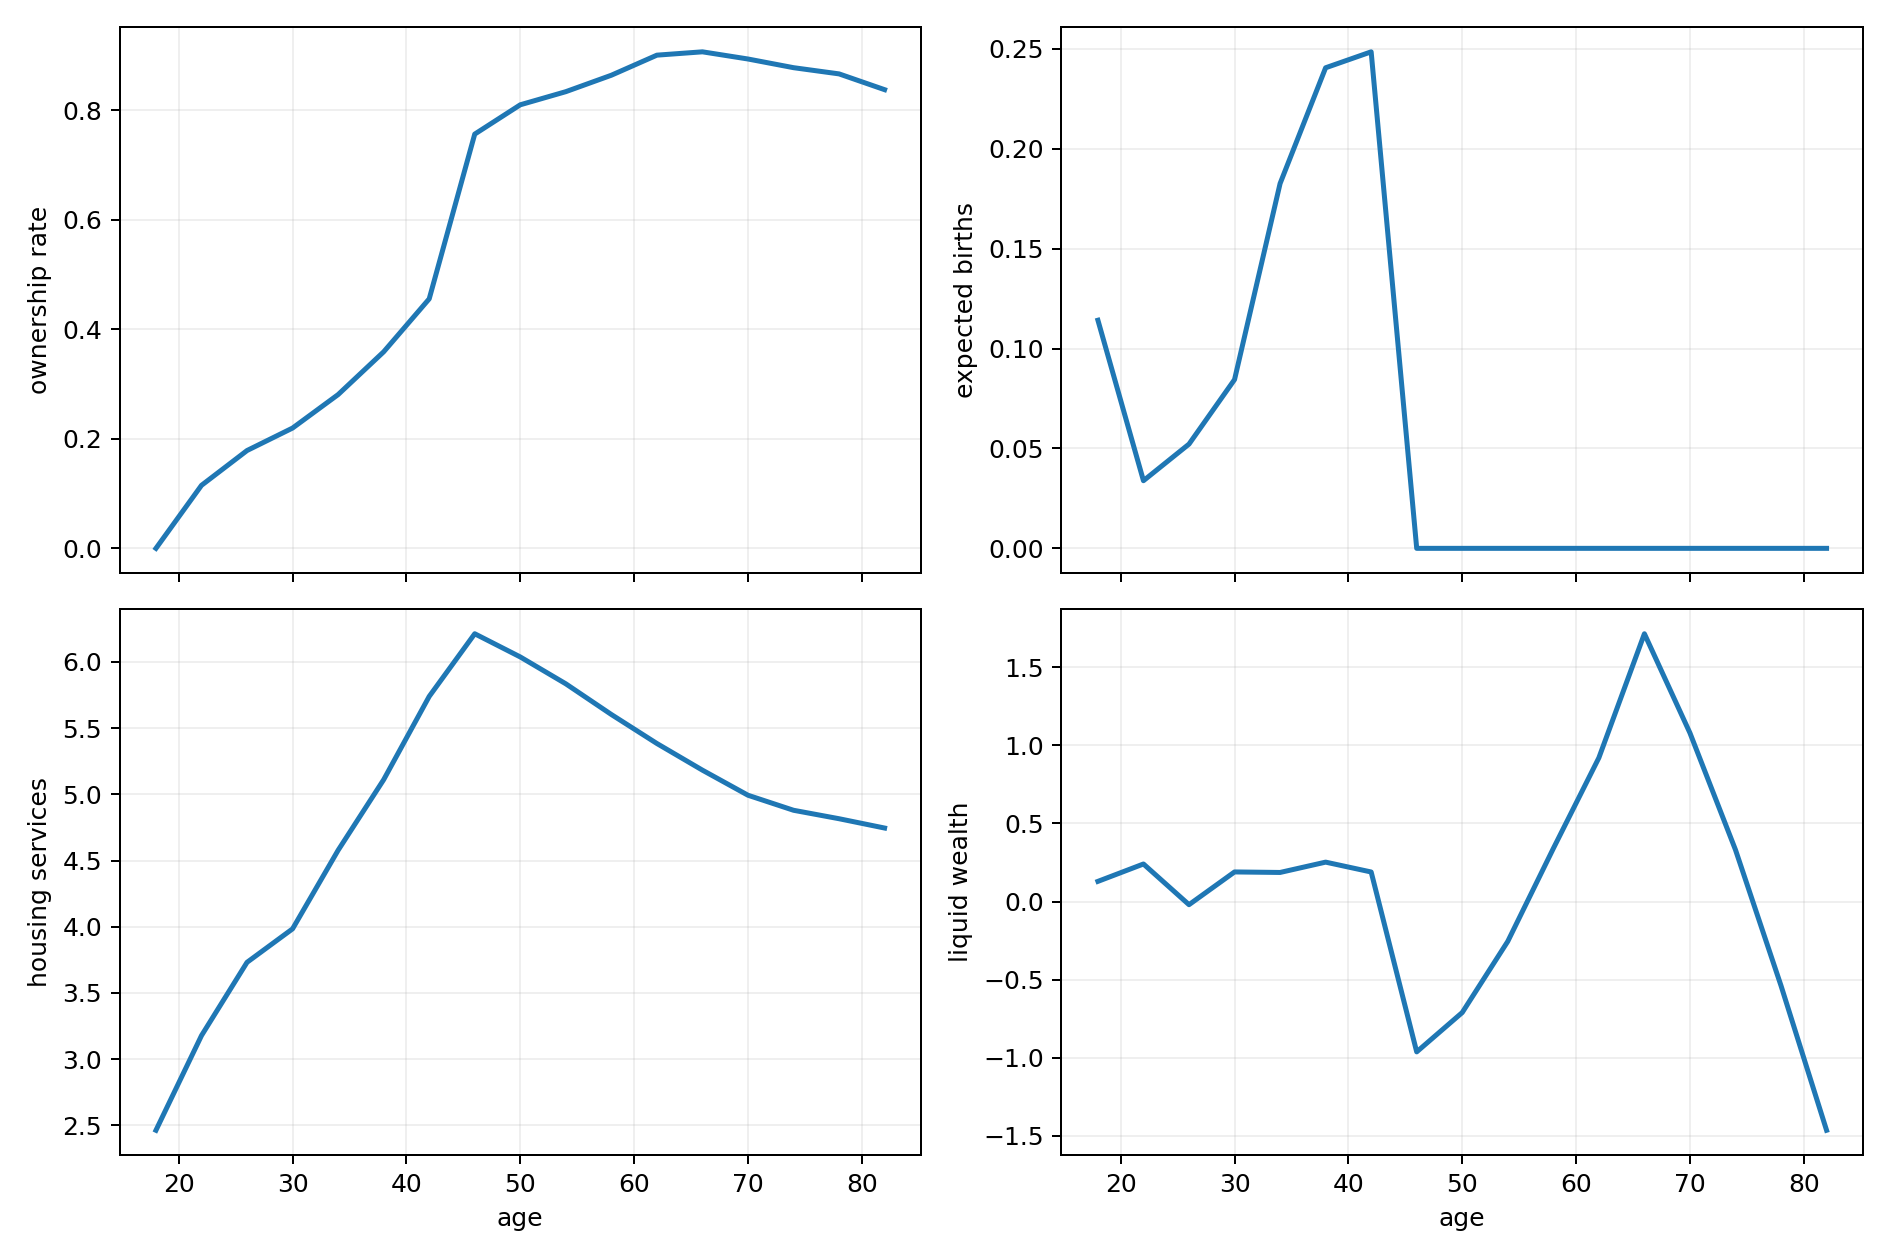
\includegraphics[width=0.97\textwidth,height=0.58\textheight,keepaspectratio]{July_26_slides_age_profiles.png}
  \begin{itemize}
    \item Ownership jumps at the last fertile age, not gradually before it.
    \item Births cluster at age $33$ with a spike at the deadline; in the data they peak near $27$.
    \item Liquid wealth drops sharply at the family purchase, as households lever up to the limit.
  \end{itemize}
  The remaining fit problem is timing: the model buys and gives birth too late.
\end{frame}

% 15
\begin{frame}{What the Misses Are Telling Us}
  \begin{tabularx}{\textwidth}{>{\raggedright\arraybackslash}p{0.45\textwidth}>{\raggedright\arraybackslash}X}
  \toprule
  diagnosed miss & fix designed, not yet adopted\\
  \midrule
  Old-age ownership is $0.892$ against $0.764$ in the data. & Give old owners a health, mortality, or downsizing exit.\\
  Young ownership is $0.226$ against $0.341$, and young wealth is $0.354$ against $0.179$. & Fix fertility timing, rather than re-searching the same parameter box.\\
  Childlessness by income runs the wrong way. & Add a child time cost, so children cost time as well as goods and rooms.\\
  \bottomrule
  \end{tabularx}

  {\small The misses hang together: late fertility and no old-age exit are doing work that no parameter can do cleanly.}
\end{frame}

% 16
\begin{frame}{The Access Gap Shows Up in the Calibration}
  \begin{itemize}
    \item Among fertile renters constrained by the rental size limit, $\zeta/q=1.28$.
    \item These renters value family space at $2.3\times$ market user cost.
    \item A share $0.734$ of the fertility-response mass sits on households with $\zeta>0$.
    \item The share is robust to numerical resolution, to how the targets are weighted, and to the owner ladder.
  \end{itemize}
  This is the equal-scaling prediction in the calibrated model: fertility exposure rises with the normalized gap $\zeta_i^m/(c_i^m-\chi n_i^m)$.
\end{frame}

% 17
\begin{frame}{Births Trigger the Purchase at the Deadline}
  \centering
  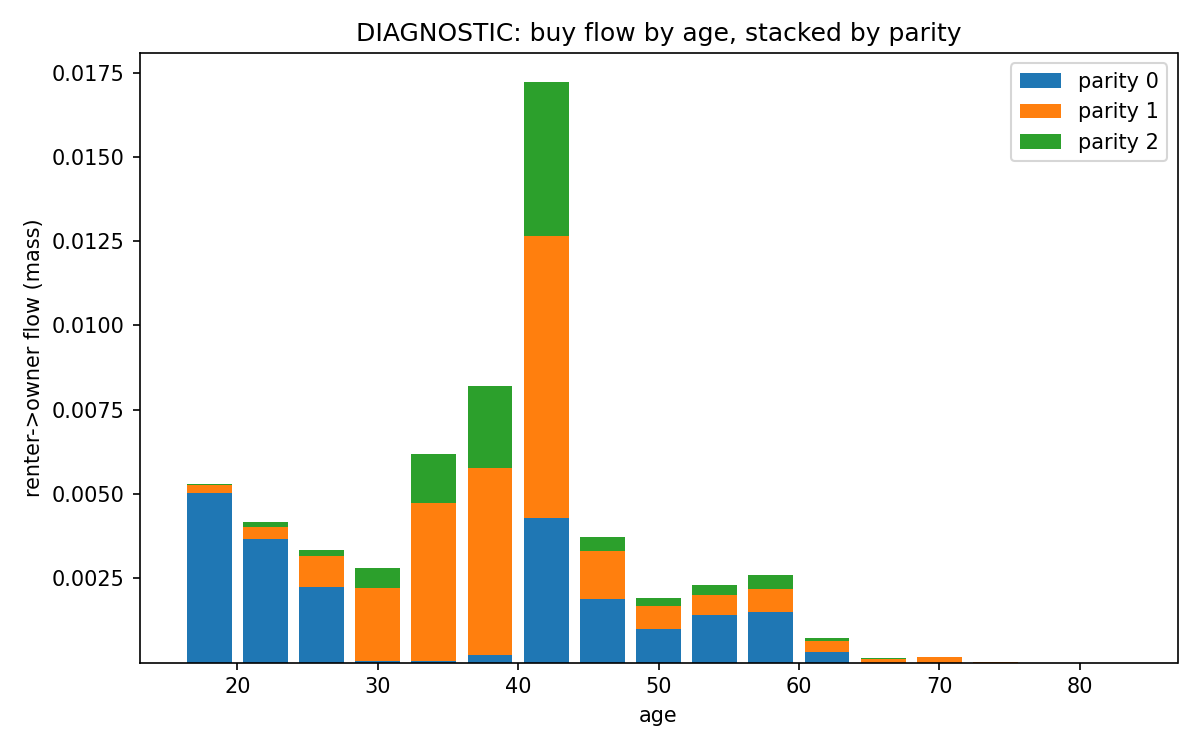
\includegraphics[width=0.88\textwidth,height=0.56\textheight,keepaspectratio]{July_26_slides_buy_flow_by_age_parity.png}
  \begin{itemize}
    \item About $29\%$ of the age-$42$ cohort buys in that single period.
    \item Seven in ten of these buyers are parents, and half have a newborn.
    \item Buyers arrive with slack: the average one is about $10$ wealth-grid cells above its down-payment threshold.
  \end{itemize}
  The purchase margin is a birth-timing margin, not slow saving finally crossing the constraint.
\end{frame}

% 18
\begin{frame}{Who Holds the Family-Sized Stock}
  The calibrated allocation gives the empirical face of the misallocation result:
  \[
  \begin{array}{lr}
  \toprule
  \text{holder group} & \text{share of rooms}\ge6\text{ stock}\\
  \midrule
  \text{post-fertile households} & 87\%\\
  \text{households with no kids at home} & 72\%\\
  \text{fertile parents} & 12.6\%\\
  \bottomrule
  \end{array}
  \]
  The households with the largest measured access gap hold almost none of the family-sized owner stock. This is the planner-equilibrium comparison, stated as an accounting fact about the calibrated economy.
\end{frame}

% 19
\begin{frame}{A Price Instrument Capitalizes but Barely Moves Births}
  \begin{itemize}
    \item Consider a $2\%$ tax on large homes.
    \item Large-home prices fall by $12.3\%$.
    \item Fertility hardly moves: $\Delta \mathrm{TFR}=+0.004$.
    \item The response is robust to numerical resolution, to the housing menu, and to the weighting of targets.
  \end{itemize}
  A pure price instrument capitalizes into house prices; it does not create births.
\end{frame}

% 20
\begin{frame}{Birth-Linked Purchase Grants Move Fertility}
  A grant paid at a birth-linked purchase raises fertility, and the response grows with the size of the grant:
  \[
  \begin{array}{cc}
  \toprule
  \text{grant size} & \Delta \mathrm{TFR}\\
  \midrule
  0.1 & +0.01\\
  0.4 & +0.13\\
  0.58 & +0.26\\
  1.0 & +0.49\\
  \bottomrule
  \end{array}
  \]
  Prices barely move --- large-home prices rise about $1\%$.
  \begin{itemize}
    \item One caveat: a small conditional grant can pull purchases back before the birth, delaying them through anticipation.
  \end{itemize}
  Grants move the birth margin because they relax the owner financing gap $\zeta_i^{O,F}$.
\end{frame}

% 21
\begin{frame}{A Package That Decentralizes the Reallocation}
  Tax the incumbent stock and spend the revenue on young buyers' access:
  \[
  \text{large-home tax}+\text{birth-linked purchase grant}
  \quad\Rightarrow\quad
  \Delta \mathrm{TFR}=+0.15,\quad
  \Delta p_{\text{large}}=-11\%.
  \]
  The tax lowers what incumbents will pay to keep large units; the grant closes the young side's financing gap at the birth margin. Revenue-funded, it is the decentralized version of the planner's move --- and it works through access, not price.
\end{frame}

% 22
\begin{frame}{The Bridge, in Three Numbers}
  \begin{enumerate}
    \item Access: fertile renters at the cap have $\zeta/q=1.28$, and $0.734$ of the fertility-response mass sits on households with $\zeta>0$.
    \item Allocation: $87\%$ of the family-sized stock is held by post-fertile households.
    \item Policy: the tax-funded access transfer raises TFR by $0.15$ while cutting large-home prices $11\%$.
  \end{enumerate}
  The same object $\zeta$ measures fertility exposure and stock misallocation, and the package is the decentralized version of the planner's reallocation.
\end{frame}

% 23
\begin{frame}{Where This Version Falls Short}
  \begin{itemize}
    \item Several parameters sit at their search bounds.\footnote{Eight of the $13$ estimated parameters are at or against a bound at the current calibration --- evidence that the parameter space is compensating for missing mechanisms, not a failure of the search.}
    \item Fertility is mistimed: births cluster at $33$, against a data peak near $27$.
    \item Planned extension: a child time cost, so children are priced partly in foregone income.
    \item Planned extensions: an old-age exit margin, and childlessness targets consistent with the estimand.
  \end{itemize}
  These belong in the draft as honest limitations, not as settled calibration details.
\end{frame}

% 24
\begin{frame}{Conclusion}
  \alert{[PLACEHOLDER: conclusion]}
  \begin{itemize}
    \item {[}PLACEHOLDER: final theory sentence]
    \item {[}PLACEHOLDER: final quantitative sentence]
    \item {[}PLACEHOLDER: final policy sentence]
  \end{itemize}
\end{frame}

\end{document}
